
\lettrine[lines=3]{T}{}he string interpreter is one of the major components of the L-system, it is the final step in the process of procedural generation. The output of this stage of processing is dependant on what the L-system is representing, in this case it is responsible for interpreting the resulting string of modules, and uses this to generate the 3D models, structures and data of the resulting plant which is then rendered and simulated on the screen using the OpenGL framework. The generation of plant-life has three main stages, the first part is a turtle graphics interpreter which takes the string of modules, these modules are interpreted as a set of instructions, starting from the root of the tree and generates a skeleton made up of branch joints, similar to the techniques used in skeletal rigging in animation \cite{gregory2014game}. The joints within the tree skeleton each represent a branch segment which has some information about the properties of that segment. These segements can be used to generate the vertex, index and other data that make up the 3D models of the plant. These models can finally be passed to the renderer which renders the plant on the screen. The stages of string interpretation can be seen in figure \ref{l-system interpreter} below. 

\begin{figure}[htbp]
	{\centering
		\vspace{7px}
		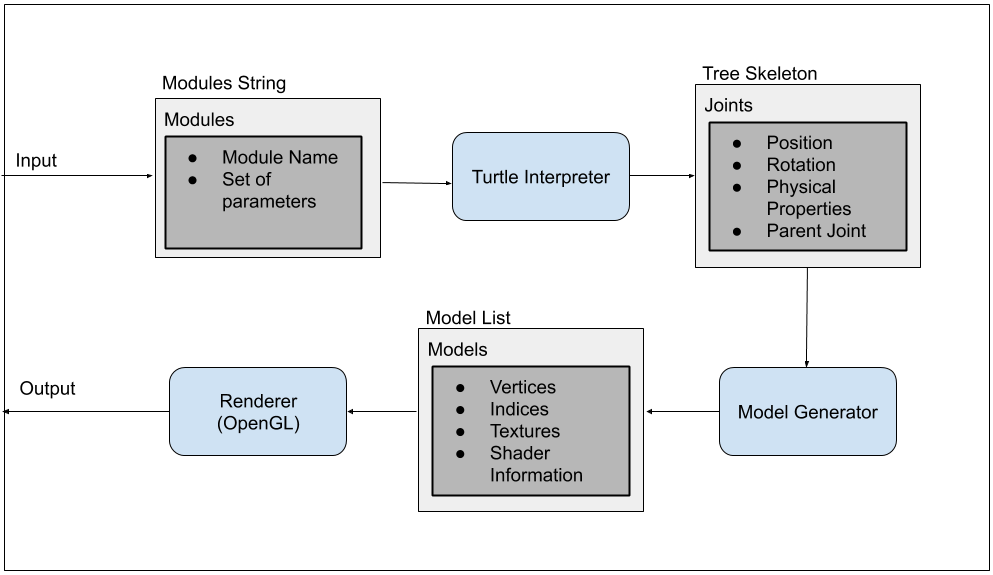
\includegraphics[scale=0.4]{Diagrams/L-systemInterpreter.png}
		\caption{Diagram of the stages of L-system interpretation and rendering} \label{l-system interpreter}
	}
\end{figure}

\noindent
This chapter will outline each stage in the string interpreter implementation for generating 3D models of plant structures as well as well as talking about how the interpreter is able to simulate and animation the plants movements under forces such as gravity and wind in real time. \\

\section{Turtle Graphics Interpreter}


The main job of the turtle graphics interpreter is to take the string of modules from the L-system rewriter and interpret it as a list of turtle graphics instructions. These instructions generate the plants skeleton which is made up of joints, the joints that hold information as to its 3D properties of a particular segement or object. The properties are the position, orientation, physical properties as well as the parent of the joint. The information for each joint is as follows:

\begin{figure}[htbp]
	{\centering
		\vspace{7px}
		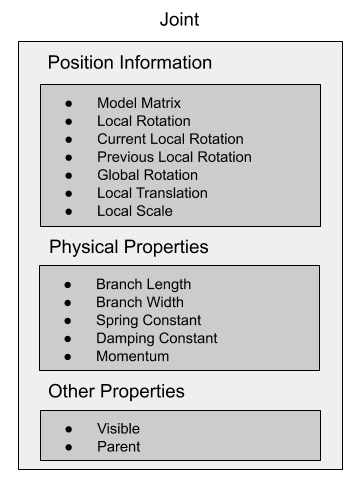
\includegraphics[scale=0.6]{Diagrams/JointDiagram.png}
		\caption{Diagram for the properties of a joint} \label{joint properties}
	}
\end{figure}

\noindent
As you can see from figure \ref{joint properties}, there is large amount of information stored for the position and orientation of each joint. This is because each rotation is stored in both a local and global space. Local space refers to the rotation of the joint relative to the joints parent rotation, this is useful as it allows the manipulation of subsequent child joints but leaving parent joints local rotation unchanged. Global space, also known as world space, is the rotation of the joint relative to the world itself this is useful for understanding the current rotation of the joint relative to the world for instance calculating the torque or force calculations due to gravity. Furthermore it is important to store both the current and previous rotations to calculate the rate of change for physics calculations.

The physical properties for each joint are the parts that will affect the model generation stage as well as the physics simulation. These include the length of the branch stemming from the joint position, the width of the branch, the spring constant or stiffness of the branch, the damping constant for slowing down the branch oscillation and the current momentum of the branch. 

Take the string of modules \say{F(1)[/(90)F(1)$\backslash$ (90)F(1)]-(90)F(1)+(90)F(1)}, the alphabet is made up of seven unique modules F, /, $\backslash$, [, ], + and -. According to the as discussed in previous chapters the \say{F} symbol represents a move forward, and \say{+}, \say{-}, \say{/}, \say{$\backslash$} symbolize different rotations, and the \say{[} and \say{]} represent save and load state respecively. The aforementioned symbols each have a single parameter except the load and save state. It is the turtle graphics interpreters job to understand what these parameters are and how to interpret them. In this case all of the \say{F} modules have the parameter value of 1, and all of the rotation modules have the parameter of 90. These are interpreted as the distance to move forward and the angle to rotate respectively. This interpretation can be represented with the joint structure shown below:

\begin{figure}[htbp]
	{\centering
		\vspace{7px}
		\setlength{\fboxrule}{1pt}
		\fbox{
			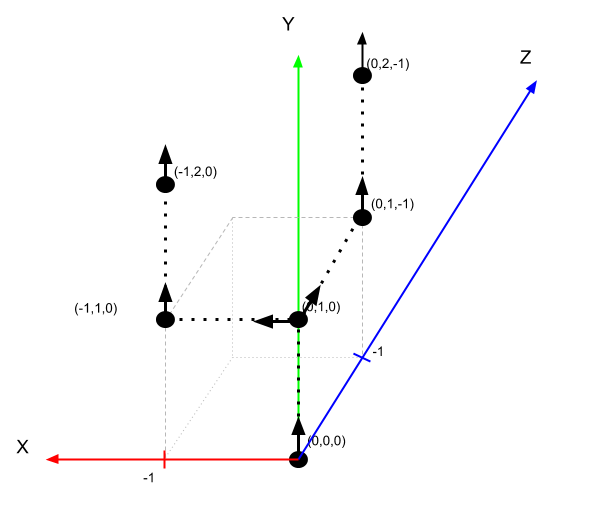
\includegraphics[scale=0.4]{Diagrams/SkeletonJoints.png}
		}
		\caption{Diagram of a simple plant skeleton with joint position and orientation.}
	}
\end{figure}

\FloatBarrier


\section{Model Generator}

\begin{flushleft}

Modeling the branches of a plant is one of the most important parts for the overall look and feel of that plant that is being generated. The L-system described in the previous sections is able to describe the details about the plants structure, for instance the position, width, length, weight and other important information. The job of the model generator is to take this information and intelligently generate the models vertices, normals, texture coordinates and other information that can then be provided to the OpenGL renderer and finally to the GPU to be rendered on the screen. \\

\vspace{5mm}

The simplest way to generate a model for a branching structure of a plant would be to take a number of cylinders, and to rotate and stack them according to each joints position in 3D space. The up side to this approach is that every branch within the plant shares the same object model, depending on the position, rotation and scale of the branch the relavent matrix transforms can be applied. In this way we are able to represent the overall branching structure of the plant. However, there is a problem which is pointed out by Baele and Warz\'{e}e "The branches junction causes a continuity problem: to simply stack up cylinders generates a gap" \cite{baele2005real}. This can be shown in the figure below:

\FloatBarrier

\begin{figure}[htbp]
	{\centering
		\vspace{7px}
		\setlength{\fboxrule}{1pt}
		\fbox{
			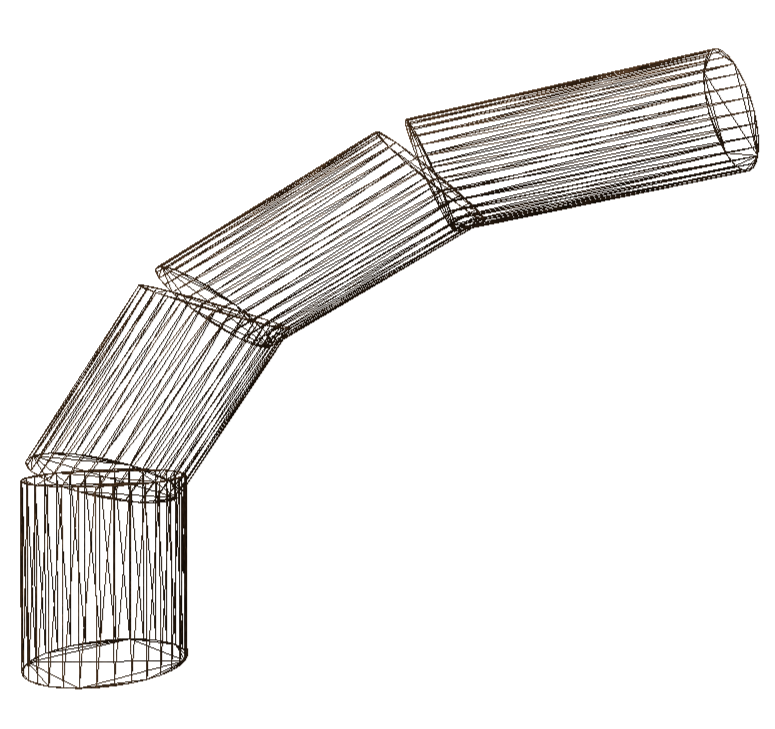
\includegraphics[scale=0.2]{Diagrams/stackedBranchesMesh.png}
		}
		\caption{Example of the continuity problem faced with stacked branching with a 25$^{\circ}$ bend per joint.}
	}
\end{figure}

\FloatBarrier

\vspace{5mm}


\vspace{5mm}

This simple method of stacking cylinders gives a reasonable looking tree structure and it is usually good enough when the angles of branches are not more than about 25$^{\circ}$ and the size of the branches do not change. However for a much more convincing tree structure we will want to do better than this. The logical next step would be to actively link the branch segments together.

\FloatBarrier

\begin{figure}[htbp]
	{\centering
		\vspace{7px}
		\setlength{\fboxrule}{1pt}
		\fbox{
			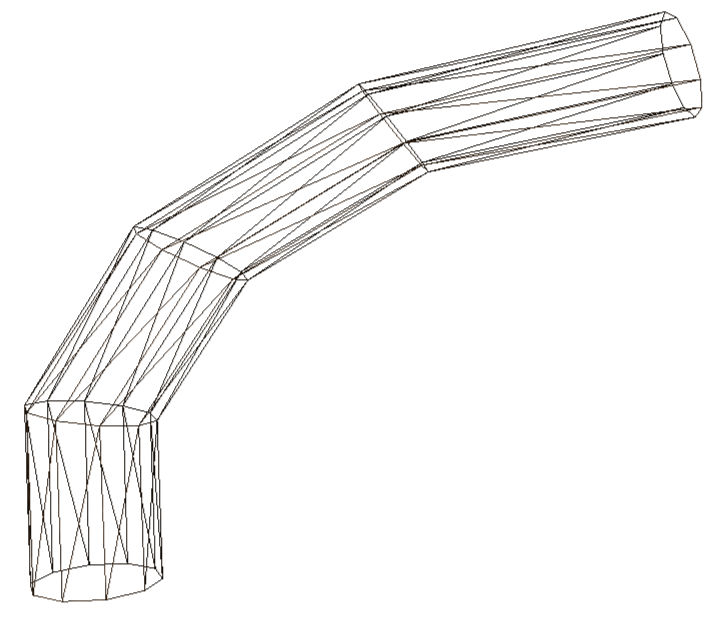
\includegraphics[scale=0.2]{Diagrams/linkedBranchesMesh.png}
		}
		\caption{Example of linked branching with a 25$^{\circ}$ bend per joint.}
	}
\end{figure}

\FloatBarrier

\end{flushleft}

\section{Renderer}

\begin{flushleft}


\end{flushleft}

\section{Displaying the L-system Instructions} \label{Display L-system Instructions}

\subsection{Basic 2D L-systems} 

There are a number of fractal geometry that have become well known particularly with regards to how they can seemingly imitate nature \cite{mandelbrot1982fractal}. Particularly with the geometry such as the Koch snowflake which can be represented using the following L-system.

\begin{figure}[htbp]
	\raggedright
	\textbf{\underline{Koch Curve:}} \\
	\#n = 4; \\
	\#define r 90; \\
	\#w : F(1); \\
	\#p1 : F(x) : * : F(x)+(r)F(x)-(r)F(x)-(r)F(x)+(r)F(x);\\
	{\centering
		\vspace{7px}
		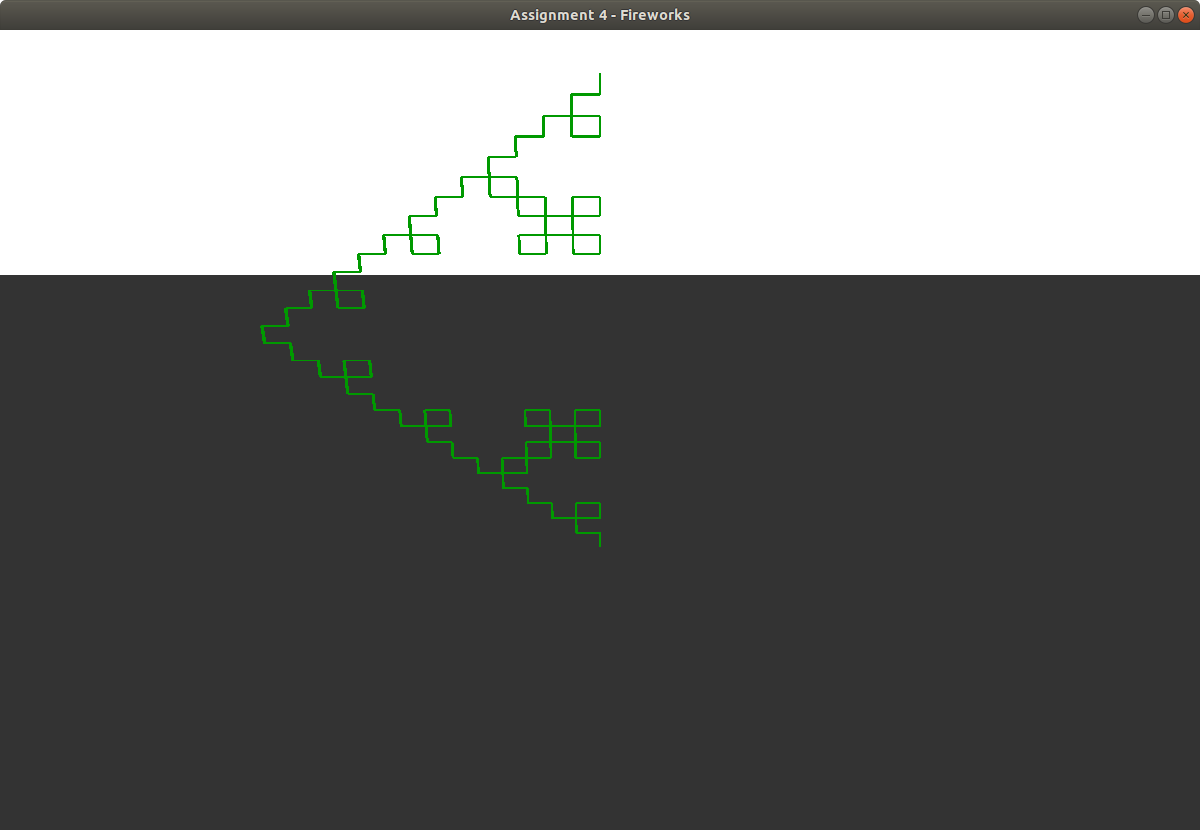
\includegraphics[scale=0.15]{KochCurve/KochCurve04.png}
		\caption{Koch Curve.}
	}
\end{figure}
\begin{figure}[htbp]
	\raggedright
	\textbf{\underline{Sierpinski Triangle:}} \\
	\#n = 4;\\
	\#define r 60;\\
	\#w : F(1);\\
	\#p1 : F(x) : * : X(x)-(r)F(x)-(r)X(x);\\
	\#p2 : X(x) : * : F(x)+(r)X(x)+(r)F(x);\\
	{\centering
		\vspace{7px}
		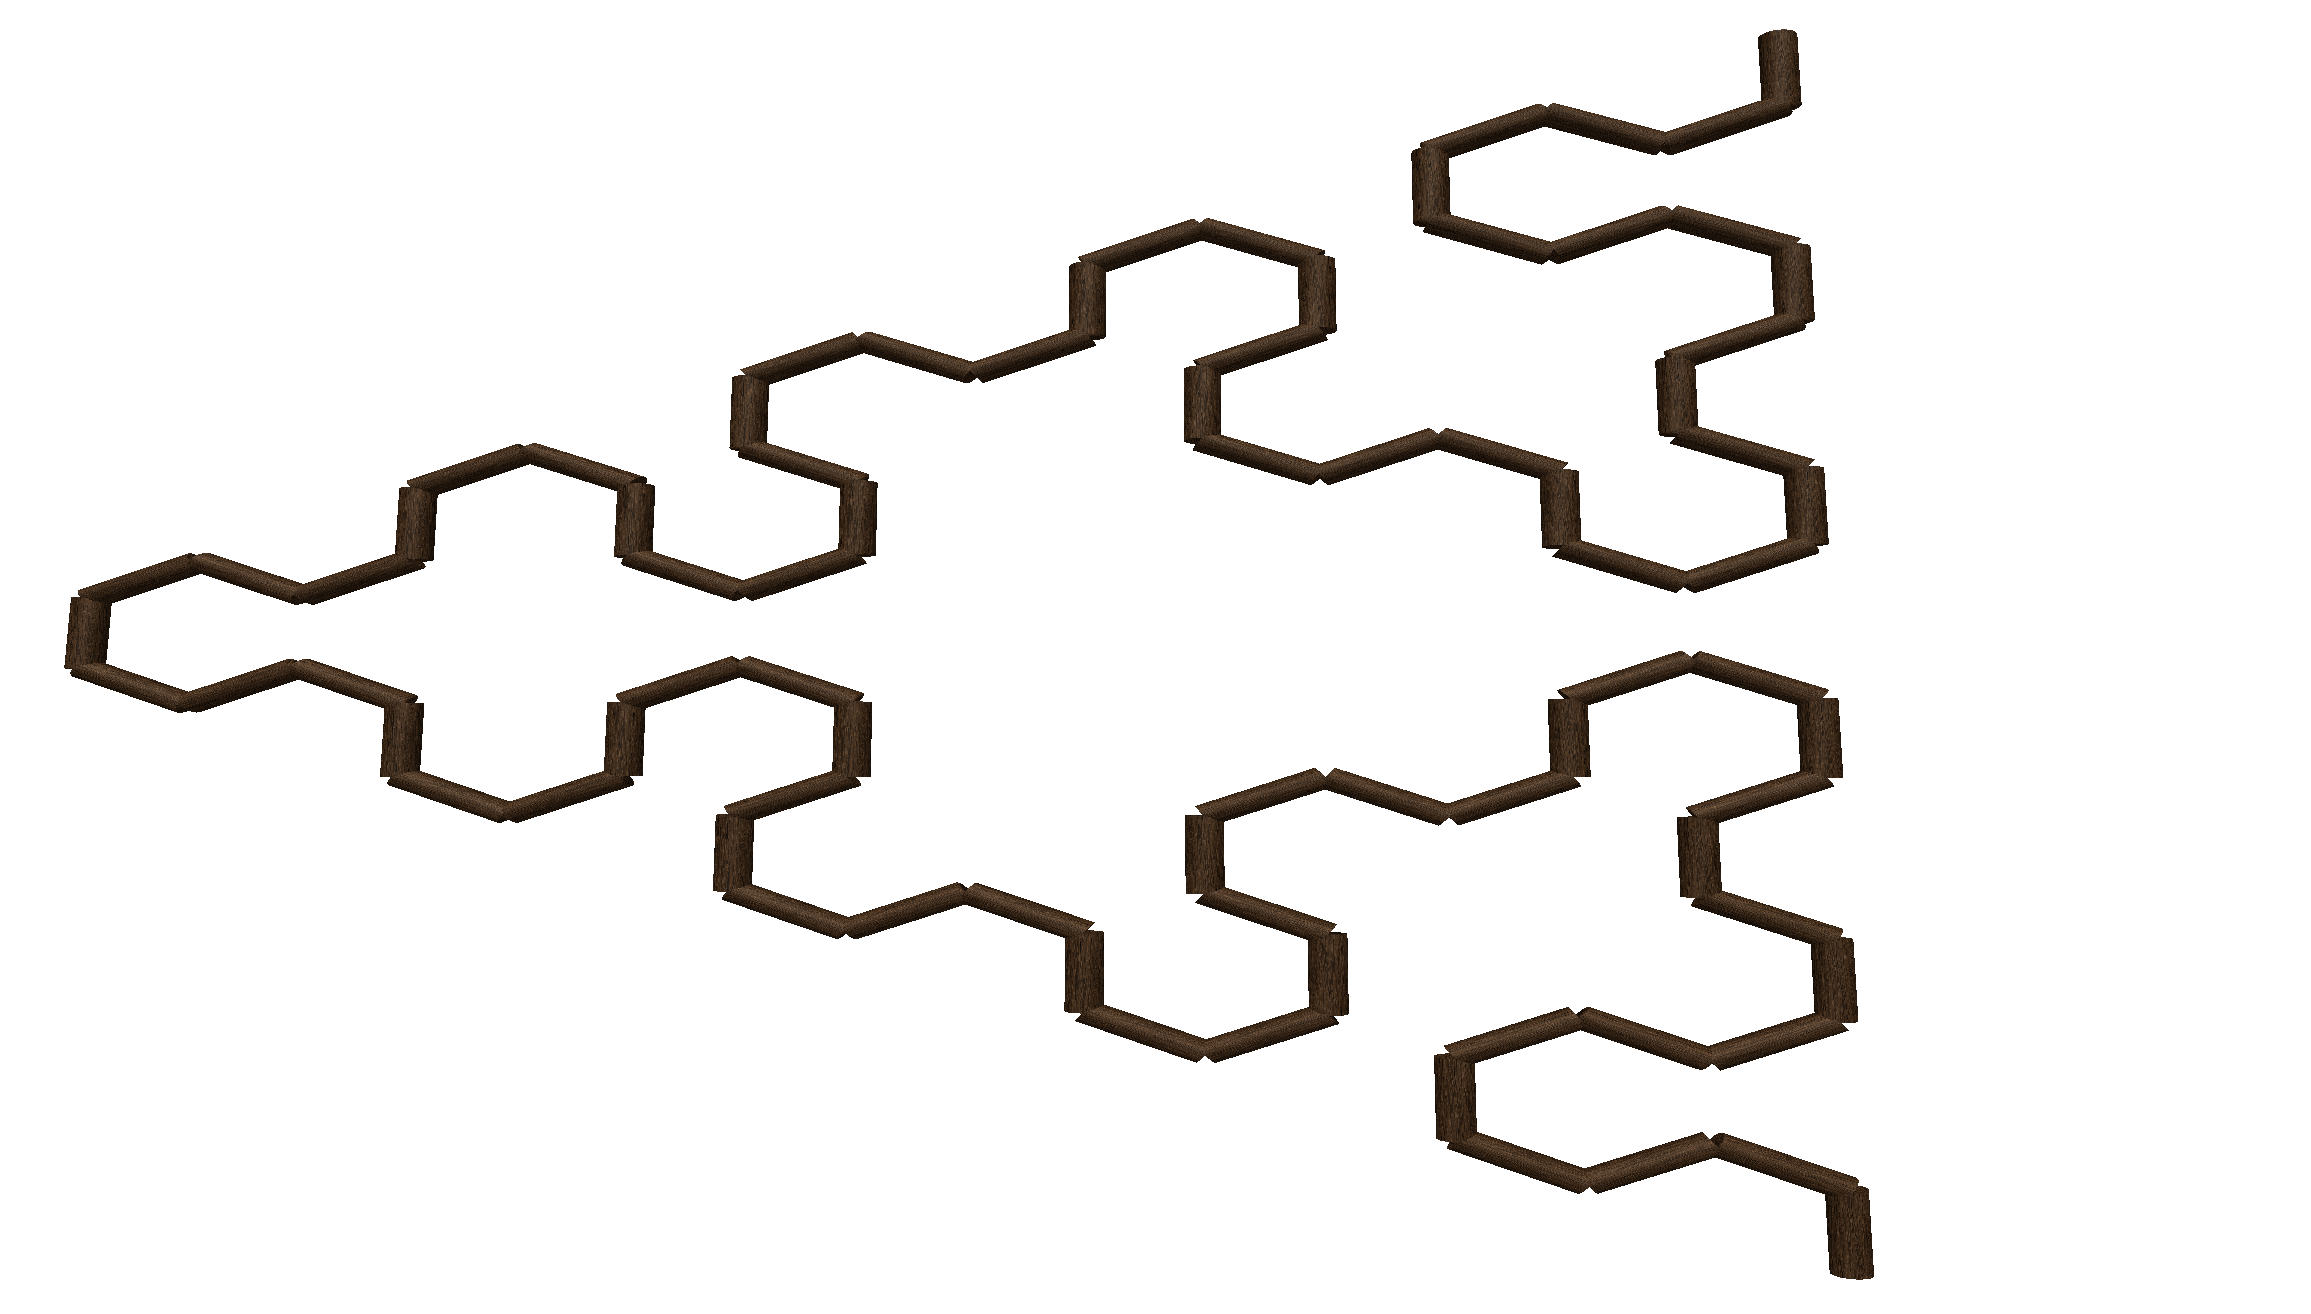
\includegraphics[scale=0.15]{SierpinskiTriangle/SierpinskiTriangle04.png}
		\caption{Sierpinski Triangle.}
	}
\end{figure}
\begin{figure}[htbp]
	\raggedright
	\textbf{\underline{Fractal Plant:}} \\
	\textbf{Alphabet:} X, F\\
	\textbf{Constants:} +, -, [, ] \\
	\textbf{Axiom:} X \\
	\textbf{Angle:} 25$^\circ$ \\
	\textbf{Rules:} \\
	X $\rightarrow$ F-[[X]+X]+F[+FX]-X\\
	F $\rightarrow$ FF \\
	{\centering
		\vspace{7px}
		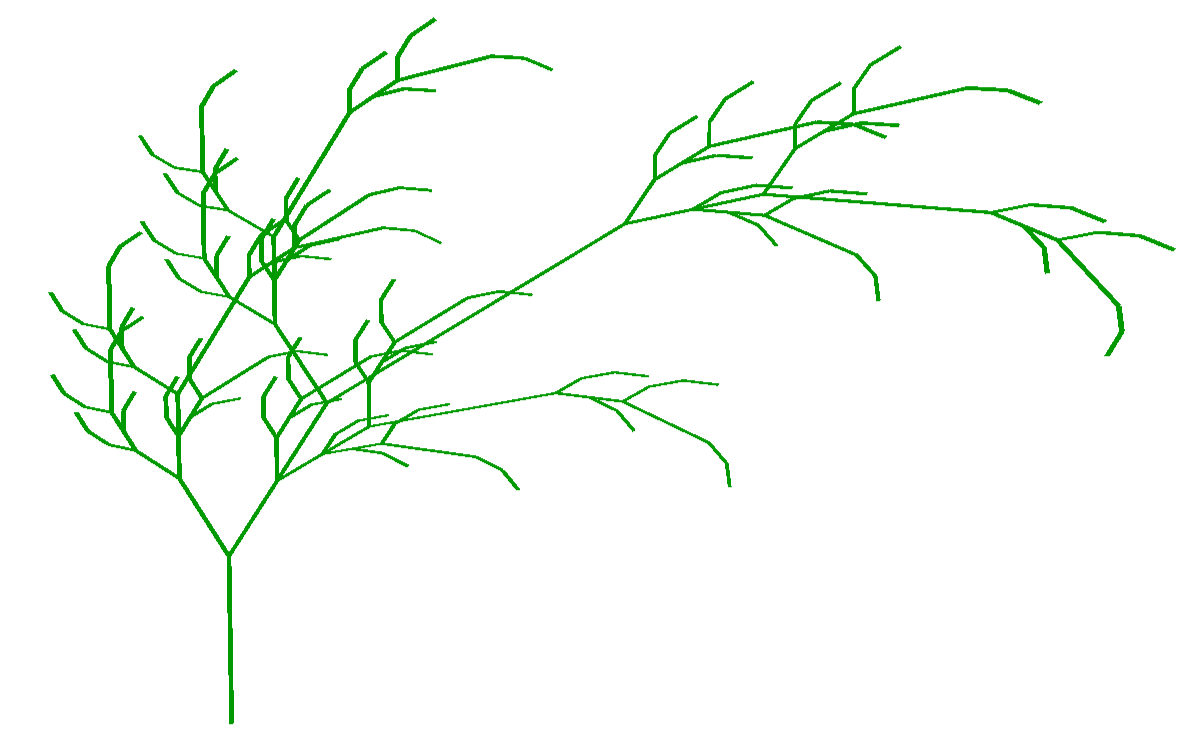
\includegraphics[scale=0.15]{FractalPlant/FractalPlant05.png}
		\caption{Fractal Plant.}
	}
\end{figure}
\begin{figure}[htbp]
	\raggedright
	\textbf{\underline{Fractal Bush:}} \\
	\textbf{Alphabet:} F\\
	\textbf{Constants:} +, -, [, ] \\
	\textbf{Axiom:} F \\
	\textbf{Angle:} 25$^\circ$ \\
	\textbf{Rules:} \\
	F $\rightarrow$ FF+[+F-F-F]-[-F+F+F]\\
	{\centering
		\vspace{7px}
		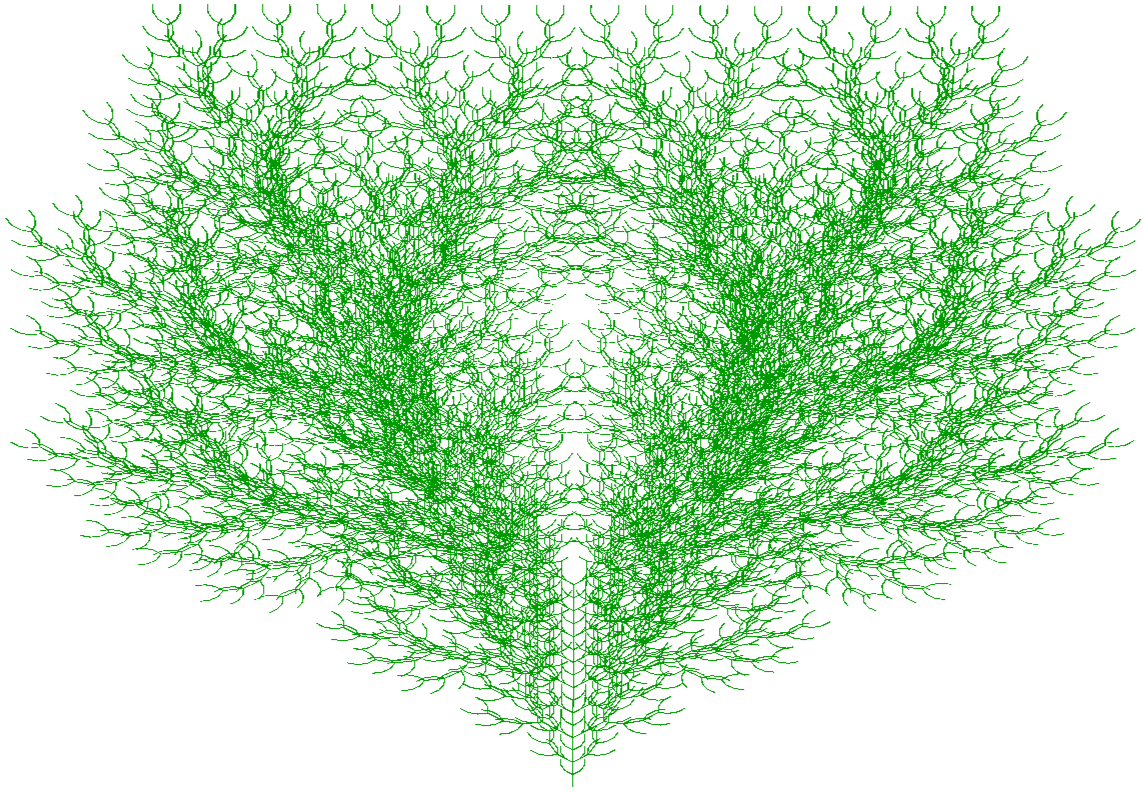
\includegraphics[scale=0.15]{FractalBush/FractalBush06.png}
		\caption{Fractal Bush.}
	}
\end{figure}

\FloatBarrier

\subsection{The Use of L-systems in 3D applications}

\begin{flushleft}

L-systems have been talked about and researched since its inception in 1968 by Aristid Lindenmayer. Over the years it's usefulness in modelling different types of plant life has been very clear, however its presence has been quite absent from any mainstream game engines for the most part, these engines relying either on digital artists skill to develop individual plants or on 3rd party software such as SpeedTree. These types of software use a multitude of different techniques however their methods are heavily rooted in Lindenmayer Systems. 

\end{flushleft}
